\section{Workflows}\label{sec:workflow}

\subsection{DevOps CI/CD pipelines}\label{subsec:ci/cd-pipelines-and-development-workflow}
As we explained while describing the infrastructure, part of our global workflow can be implemented within pipelines runners definition.
We used GitHub action and the GitHub flow to harmonise the workflow within our different type of git repositories.
GitHub allows us to define template in a single repository that can be then versioned and used in other repositories while hiding the complexity of the defined pipelines.
We also followed the GitHub flow which involve one main branch and features or hotfix branch to favor small and fast release.
As stated before other strategies can be used with an adapted development workflow.

\begin{figure}[!htbp]
    \centering
    \caption{Implementation of the GitHub Flow CI/CD workflow}
    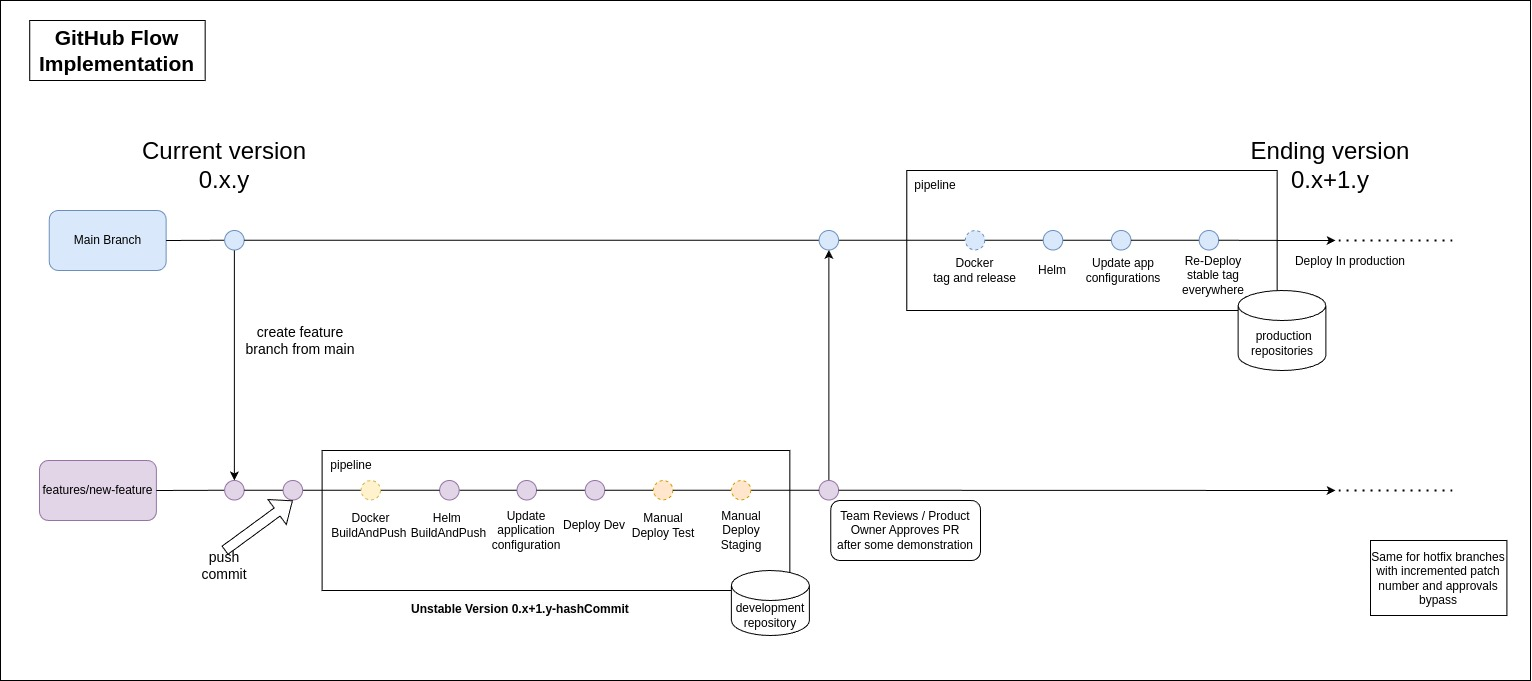
\includegraphics[scale=0.3]{images/project/cicd-workflow-p1}
    \label{fig:icd-workflow-p1}
\end{figure}

There are our development pipelines for any git repositories except for the deployment repository that are only targets.
Artifact that are not deployed but released to a directory follows the same path but are deployed as dependencies within other projects.
Airflow DAGS follows the same development workflow and are release into our previously defined git deployment repositories.

\begin{figure}[!htbp]
    \centering
    \caption{Development Team Contribution activity}
    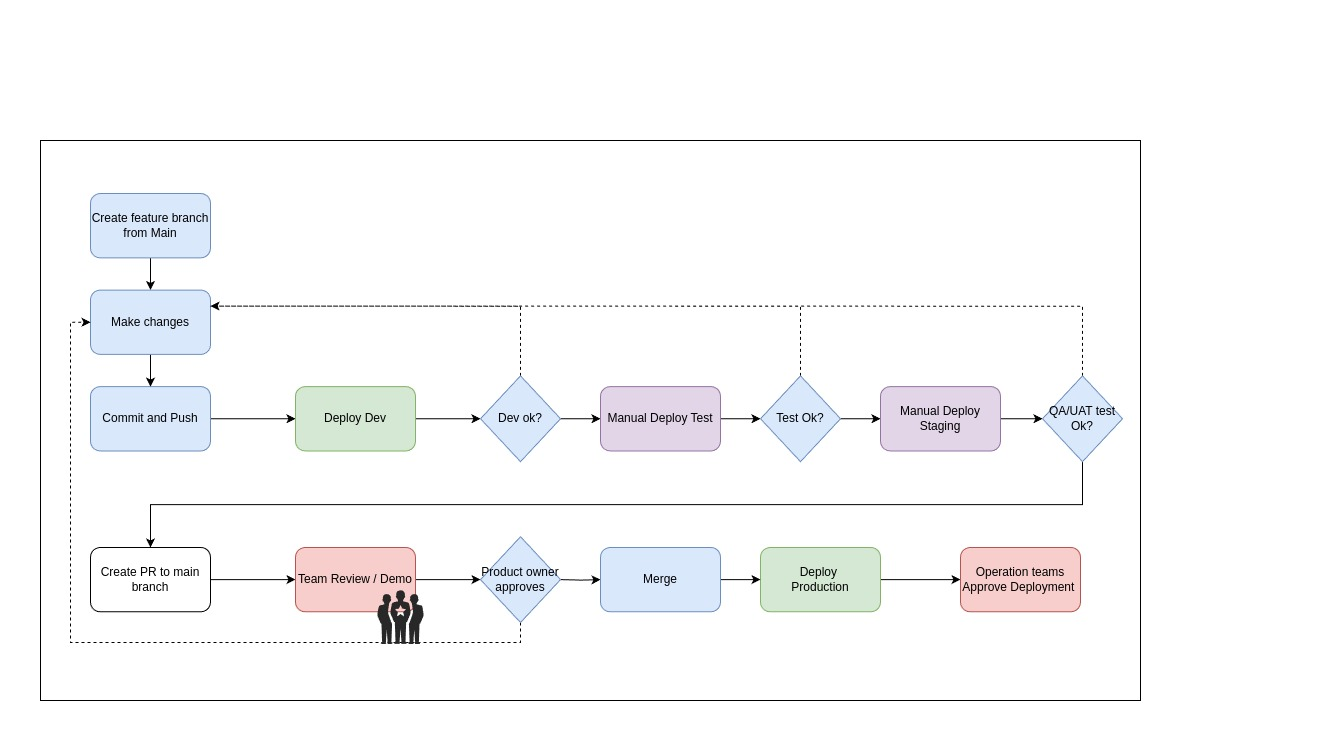
\includegraphics[scale=0.3]{images/project/cicd-workflow-p2}
    \label{fig:cd-workflow-p2}
\end{figure}


\subsection{DataOps pipelines}\label{subsec:dataops-pipelines}
Inspired by our research in the literature we create a sample DataOps pipeline that can be implemented with specific
operations.

\begin{figure}[!htbp]
    \centering
    \caption{DataOps sample workflow}
    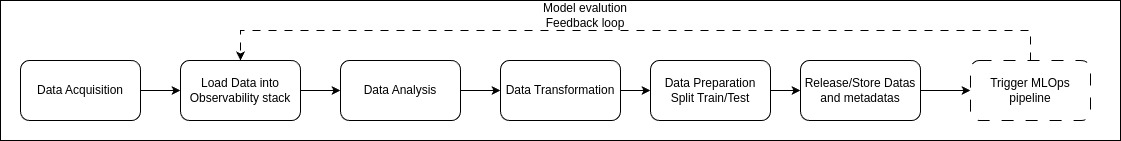
\includegraphics[scale=0.3]{images/project/dataops-workflow}
    \label{fig:dataops-workflow}
\end{figure}

It's defined in our project as an Airflow DAG and can be triggered manually in early stage of the project or
automatically when the project has enough maturity.

\subsection{MLOps pipelines}\label{subsec:mlops-pipelines}
Our MLOps pipelines are developed as Kubeflow pipelines with the possibility to trigger them from an airflow DAG
even in the early stage of the project in ensure the possibility to combined it with the DataOps pipeline to advance towards AutoML.
